The establishment of not just the concept, but also the need for a new kind of systems that, in simple terms, would allow for attesting and prove some device's location, dates back to the early beginnings of this century. 

Waters and Felten, in \cite{waters2003secure}, attempt at pioneering the design of a location-proving system by proximity that simultaneously ensures integrity and privacy. The system model assumes a fully trusted setup, fundamentally composed by two entities, a \emph{verifier} and a \emph{device}. The latter is implicitly thought to be managed by an untrusted \emph{user}, but hypothesised and expected to be tamper-resistant, and thus trusted by the verifier. The motivation behind this scenario is oriented towards practical situations in which, for instance, trusted parties lend their equipment to users and want to verify, or monitor, the equipment's location, such that it remains inside some pre-established location boundaries. The authors explicitly mention the lending of computers by universities and the wish that those devices to not leave the campuses. Home arrest monitoring systems have, as well, the need for ensuring that the ankle device, and so the person in charge, does not escape a certain location. 

\begin{figure}[ht]
    \begin{center}
    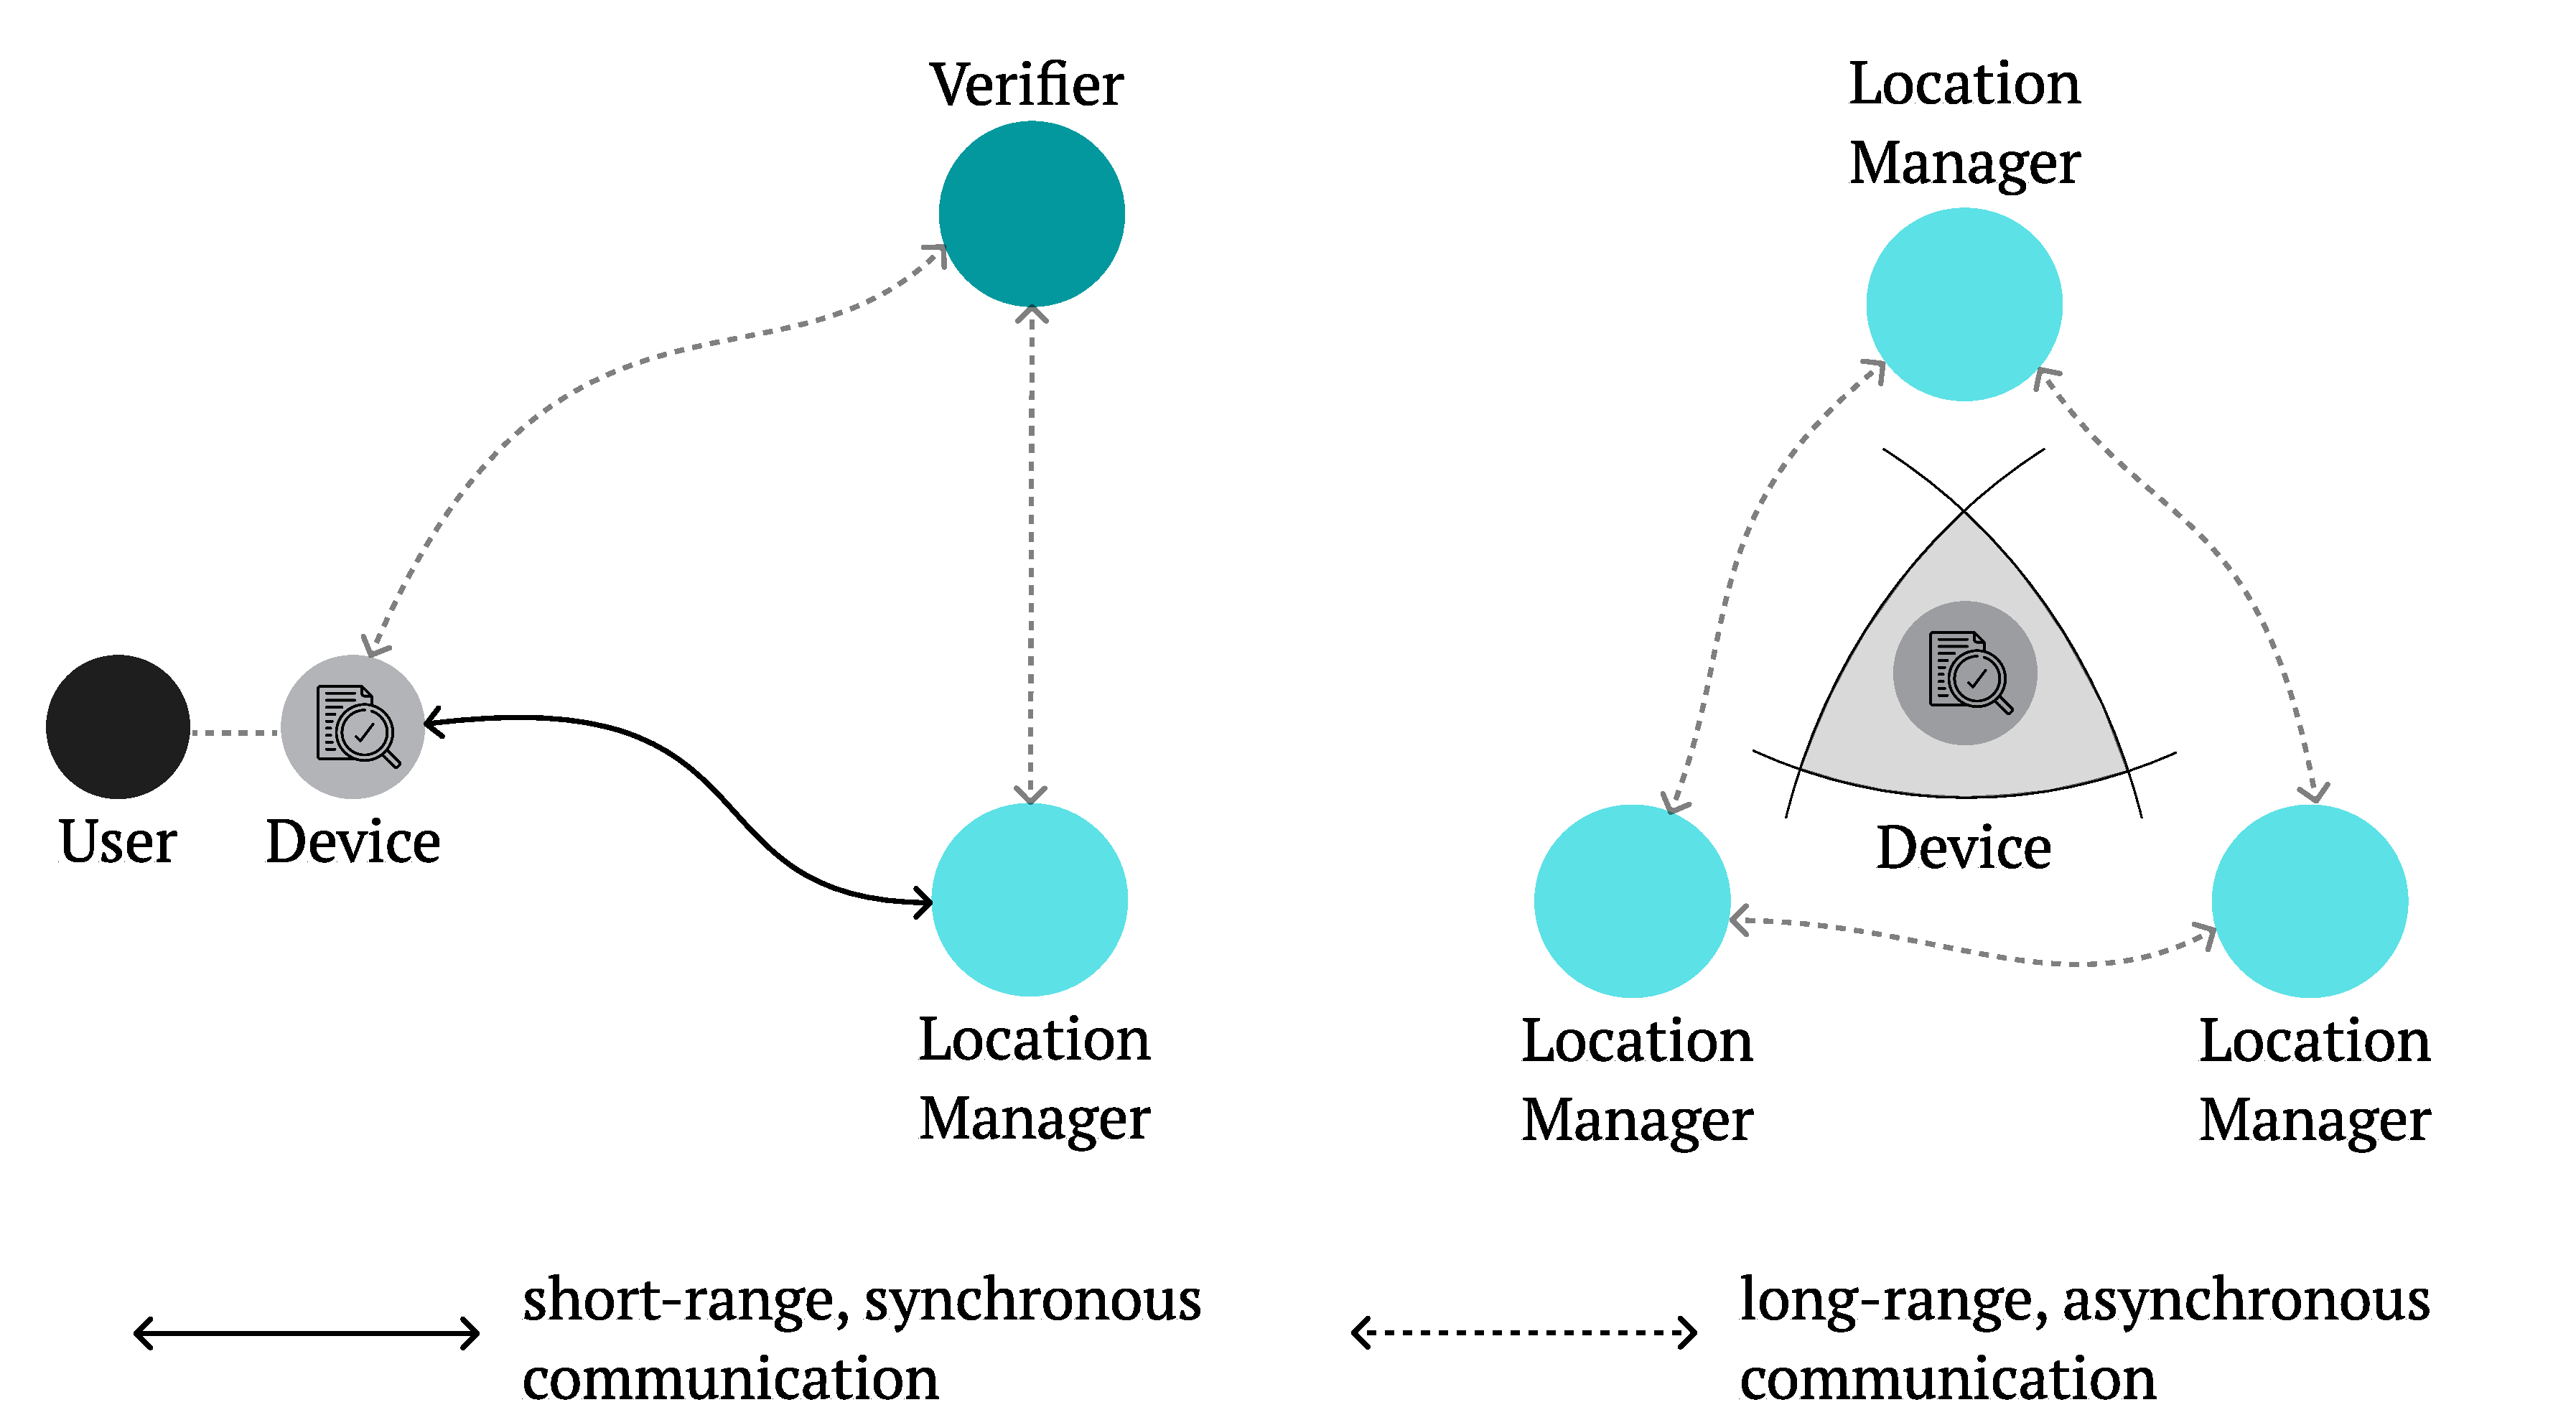
\includegraphics[width=0.9\textwidth]{trusted-centralized-pol.pdf}
    \caption{Waters and Felten's trusted and centralized \pol{} system. The device is set to accept input from an untrusted source, specifically a user, containing the identity of a nearby location manager. After receiving this input, the device will try to prove it is physically close to the designated location manager. Aiming at a more secure and precise positioning system, the device may conduct three simultaneous proofs of proximity with three location managers, to determine its relative location \cite{waters2003secure}.}
    \label{fig:trusted-centralized-pol}
    \end{center}
\end{figure}

Faced with the design and coverage unadaptability of GPS-based location systems, which do not structurally aim at serving as \pol{} enablers, the authors identify the need for small wireless networks, covering a relatively short-ranged area, via a \emph{location manager}, acting as an access point (see Figure~\ref{fig:trusted-centralized-pol}). This location manager is either set up, or distinctively trusted by the verifier. Round-trip and signal propagation latency are the metrics used, respectively, for determining the proximity of the device to the location manager and for protecting against proxy attacks~\textemdash~when a proxy device is placed near the location manager and serves as signal repeater for the original device that is somewhere else, outside the coverage area. Concretely, the work targets Wireless LAN network operators and their existing access points' infrastructure, to serve as location managers. A Public Key Infrastructure (PKI) is also proposed in order to delegate the atomic responsibility of authenticating and managing their identities to a trusted third party. Finally, the authors set down the seeds for extending their proximity proof system to a secure and moderately accurate positioning proof mechanism, with the possibility of using multiple location managers and a triangulation algorithm.

The \pol{} track was inevitably unfogged with this primordial work and location proofs were soon to be fully demystified and categorically defined. Sariou and Alec, in \cite{saroiu2009enabling}, concisely introduce the primitive concepts around \pol{} and some desired properties of an inherently secure system. However, the key contribution of their work was the delineation of a set of example applications that would benefit from \pol{} protocols. These include, but are not limited to, costumer reward systems for physical stores, location-authenticated business review systems, location-restricted web content delivery, voter's physical presence verification, among many others. A more thorough depiction of such application scenarios was left in Section~\ref{sec:background-proof-of-location-application-scenarios}.

Further protocols took inspiration from this groundwork and started shaping the landscape. Graham and Gray, in \cite{graham2009protecting}, propose a \pol{} scheme called SLVPGP that removes the need for the location manager to be trusted by the central verifier, delegating the trust to tamper-resistant modules. VeriPlace, by Luo and Hengartner \cite{luo2010veriplace}, is a complex and expensive privacy-aware location proof architecture that distributes responsibility among three types of trusted entities, taking the first step at avoiding dedicated tamper-resistant hardware. It specifically targeted the integration with Yelp\footnote{\url{https://www.yelp.com}}, a public crowd-sourced reviews system for businesses. Another worth mentioning piece of work is from Javali et al. \cite{javali2016alice}, still in a centralized and trusted stand, that adds robustness to the previous protocols by simplifying, in theoretical and practical terms, with trusted and existing Wi-Fi infrastructure, the \pol{} generation process. Finally, the work of Akand et al. \cite{akand2021privacy} is a more recent solidification attempt in the design of centralized but provably secure \pol{} systems that protect against geo-tampering attacks.

The next section will report the emergence of the first relatively distributed \pol{} protocols, taking a step further in the direction of fully decentralized and trustless systems.